\part{Towards Highly Miniaturized LED Power Systems }
\label{ch:twrd_HMLED}

\chapter{The new coming LED based lighting industry}

The appearance of light in the beginnings of the 19th century and the posterior commercialization was clearly a remarkable fact of the past history. The light bulbs contributed in two major facts that impacted peoples life . First, they enabled to have clear, reliable and safe source of light at home, extending our activity hours longer than the natural sun light. As a matter of fact we can not live without the use of artificial light.   Second, the necessity of electric power helped to develop the first electric power distribution systems. Actually, that fact can be still evidenced since people, generally our grand parents, often use the word \emph{light} when they actually are refereing electricity.

\begin{figure}[!h]
\centering
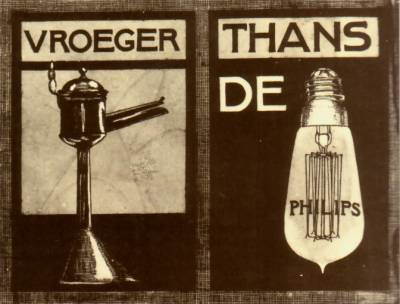
\includegraphics{./0_intro/img/1900-philips3.jpg}
\label{fig:incandescent_light_blub}
\caption{Early incandescent light bulb}
\end{figure}


From the first incandescent light bulb, the lighting industry has not had any big disruptive change to our perception of lighting till the last decade with the apparition of the LED lamps. Besides as many of us thing, it has been done a large effort to improve the efficiency of the light sources while keeping a the quality of the light as good as the incandescent light bulb. Being the florescent lamps one of the biggest contributions during the past century, beginning  to be commercialized around 1930. Later becoming a disruptive change in the lighting market with the introduction the low consumption lamps where Philips was one of the first player launching to the market the first screw-in fluorescent lamp. Although the prices of these lamps has been dropping to become commercially attractive for the costumers, their poorer color rendering factor and the longer setting time compared to the incandescent lamps prevented this lamps to be one-to-one replacement. Therefore the lighting industry has been keep without not too much attention till the introduction the LED based lamps.

\begin{figure}[!h]
\centering
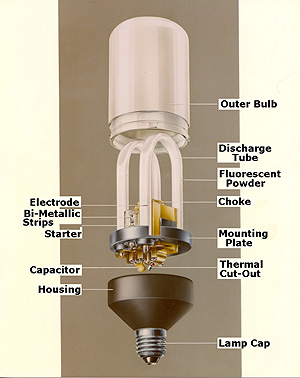
\includegraphics{./0_intro/img/phil1b.jpg}
\label{fig:philips_sl}
\caption{Components of the Philips SL compact fluorescent lamp. }
\end{figure}

The discovery of the high-efficiency blue LED ~\cite{94Nakamura} by Shuji Nakamura in 1994 enabled the quick development of the fist efficient withe LED. These early high power LEDs demonstrated that Solid State Lighting (SSL) devices  where a suitable technology for illumination. The relevance of Nakamura's work has been recognized last year being him awarded with the 2014 Nobel prize in physics. Looking farther we can also confirm the relevance of his invention since the apparition of the LED lamps, lighting is impacting again in our everyday life by changing our traditional concept of luminaries and lighting possibilities.

\begin{figure}[!h]
\centering
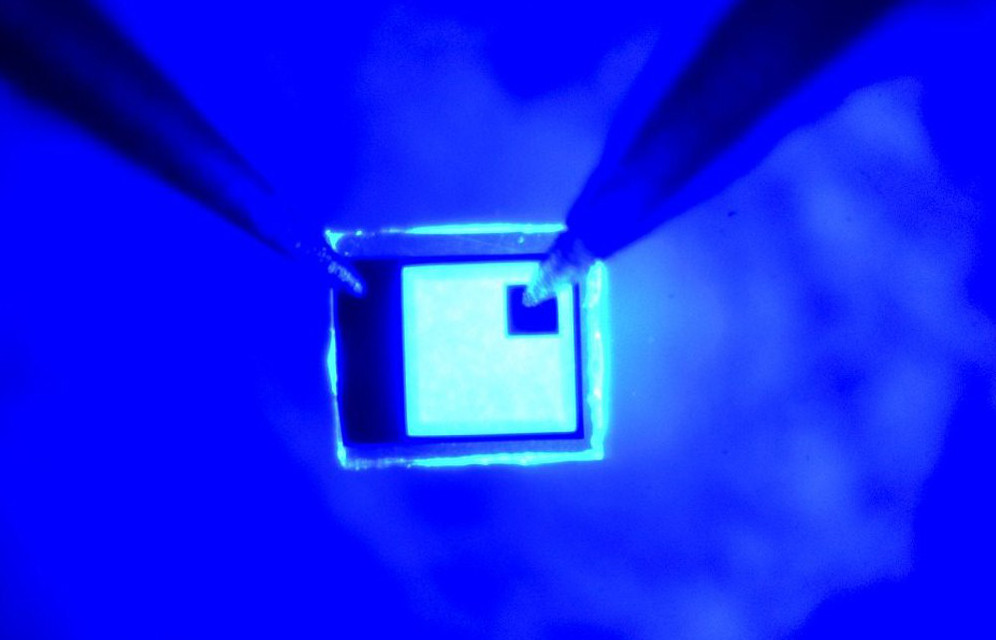
\includegraphics{./0_intro/img/10-7-14-nobel-prize-blue-led.jpg}
\label{fig:blue_LED}
\caption{Picture of a blue LED researched by Shuij Nakamura.}
\caption*{Source: \url{http://www.newsweek.com/how-blue-led-changed-world-and-won-nobel-prize-275977} }
\end{figure}

LED based lamps triggered  a frenetic rush in the lighting industry to bring that technology to the end consumers. Actually the large number of advantages of LED based lighting, or also known as Solid State Lighting (SSL), are so relevant that in the close future will replace any of the present lighting technology, that movement has been already named as the \emph{LEDification}. The principal advantages of SSL are:
\begin{description}
  \item [Efficiency] The light generation inside an LED is produced by the direct mechanism of hold-electron recombination, the supplied energy is a better use of the energy compared to the incandescent lamps. The power consumption can be up to an order of magnitude lower of an incandescent light.

  \item [Size] LEDs are tiny and flat devices, which can be considered as 2-D elements and do not need any vacuum chamber to work. They are much more flexible devices to assembly, and can easily replace the old glass made bulb design.

  \item [Color] LED light has a very narrow light spectrum, that can be used to produce directly colored light. Colored lights are becoming more popular in domestic homes becoming a piece of decoration or mood tweaking device.

  \item [Dynamics] Compared to any of the traditional sources of light LEDs have no dynamics, actually they have but it's very fast and not appreciable to the human eye. Therefore they do not have any setting time when turned on, which is not the case of CFL. The fast dynamics allows to modulate the light and transmit data without disturbing the human beings.

  \item [Lifetime] Solid State devices do not wear off, there fore they can be considered to have an infinite lifetime. In practice LEDs make use of organic phosphores, thus the light quality derates with the use, but the life expectancy of the LED is rated from 20.000 - 100.000 hours, multiplying 20 to 100 times longer that the classical light bulbs.
\end{description}

Bring the LED based lamps to the market is still a big challenge. Despite of the large number of advantages, the end consumers are still very reluctant to change generally due to the elevated costs of the new lamps, currently ranging between \$20 - \$40 for a 100W substitute compared to less than \$3 of an incandescent light. Also another issue that prevents consumers to change to the new technology is a poor light color consistency, light flickering and light dimming incompatibilities, that become really evident in low budget products. 

\begin{figure}[!h]
\centering
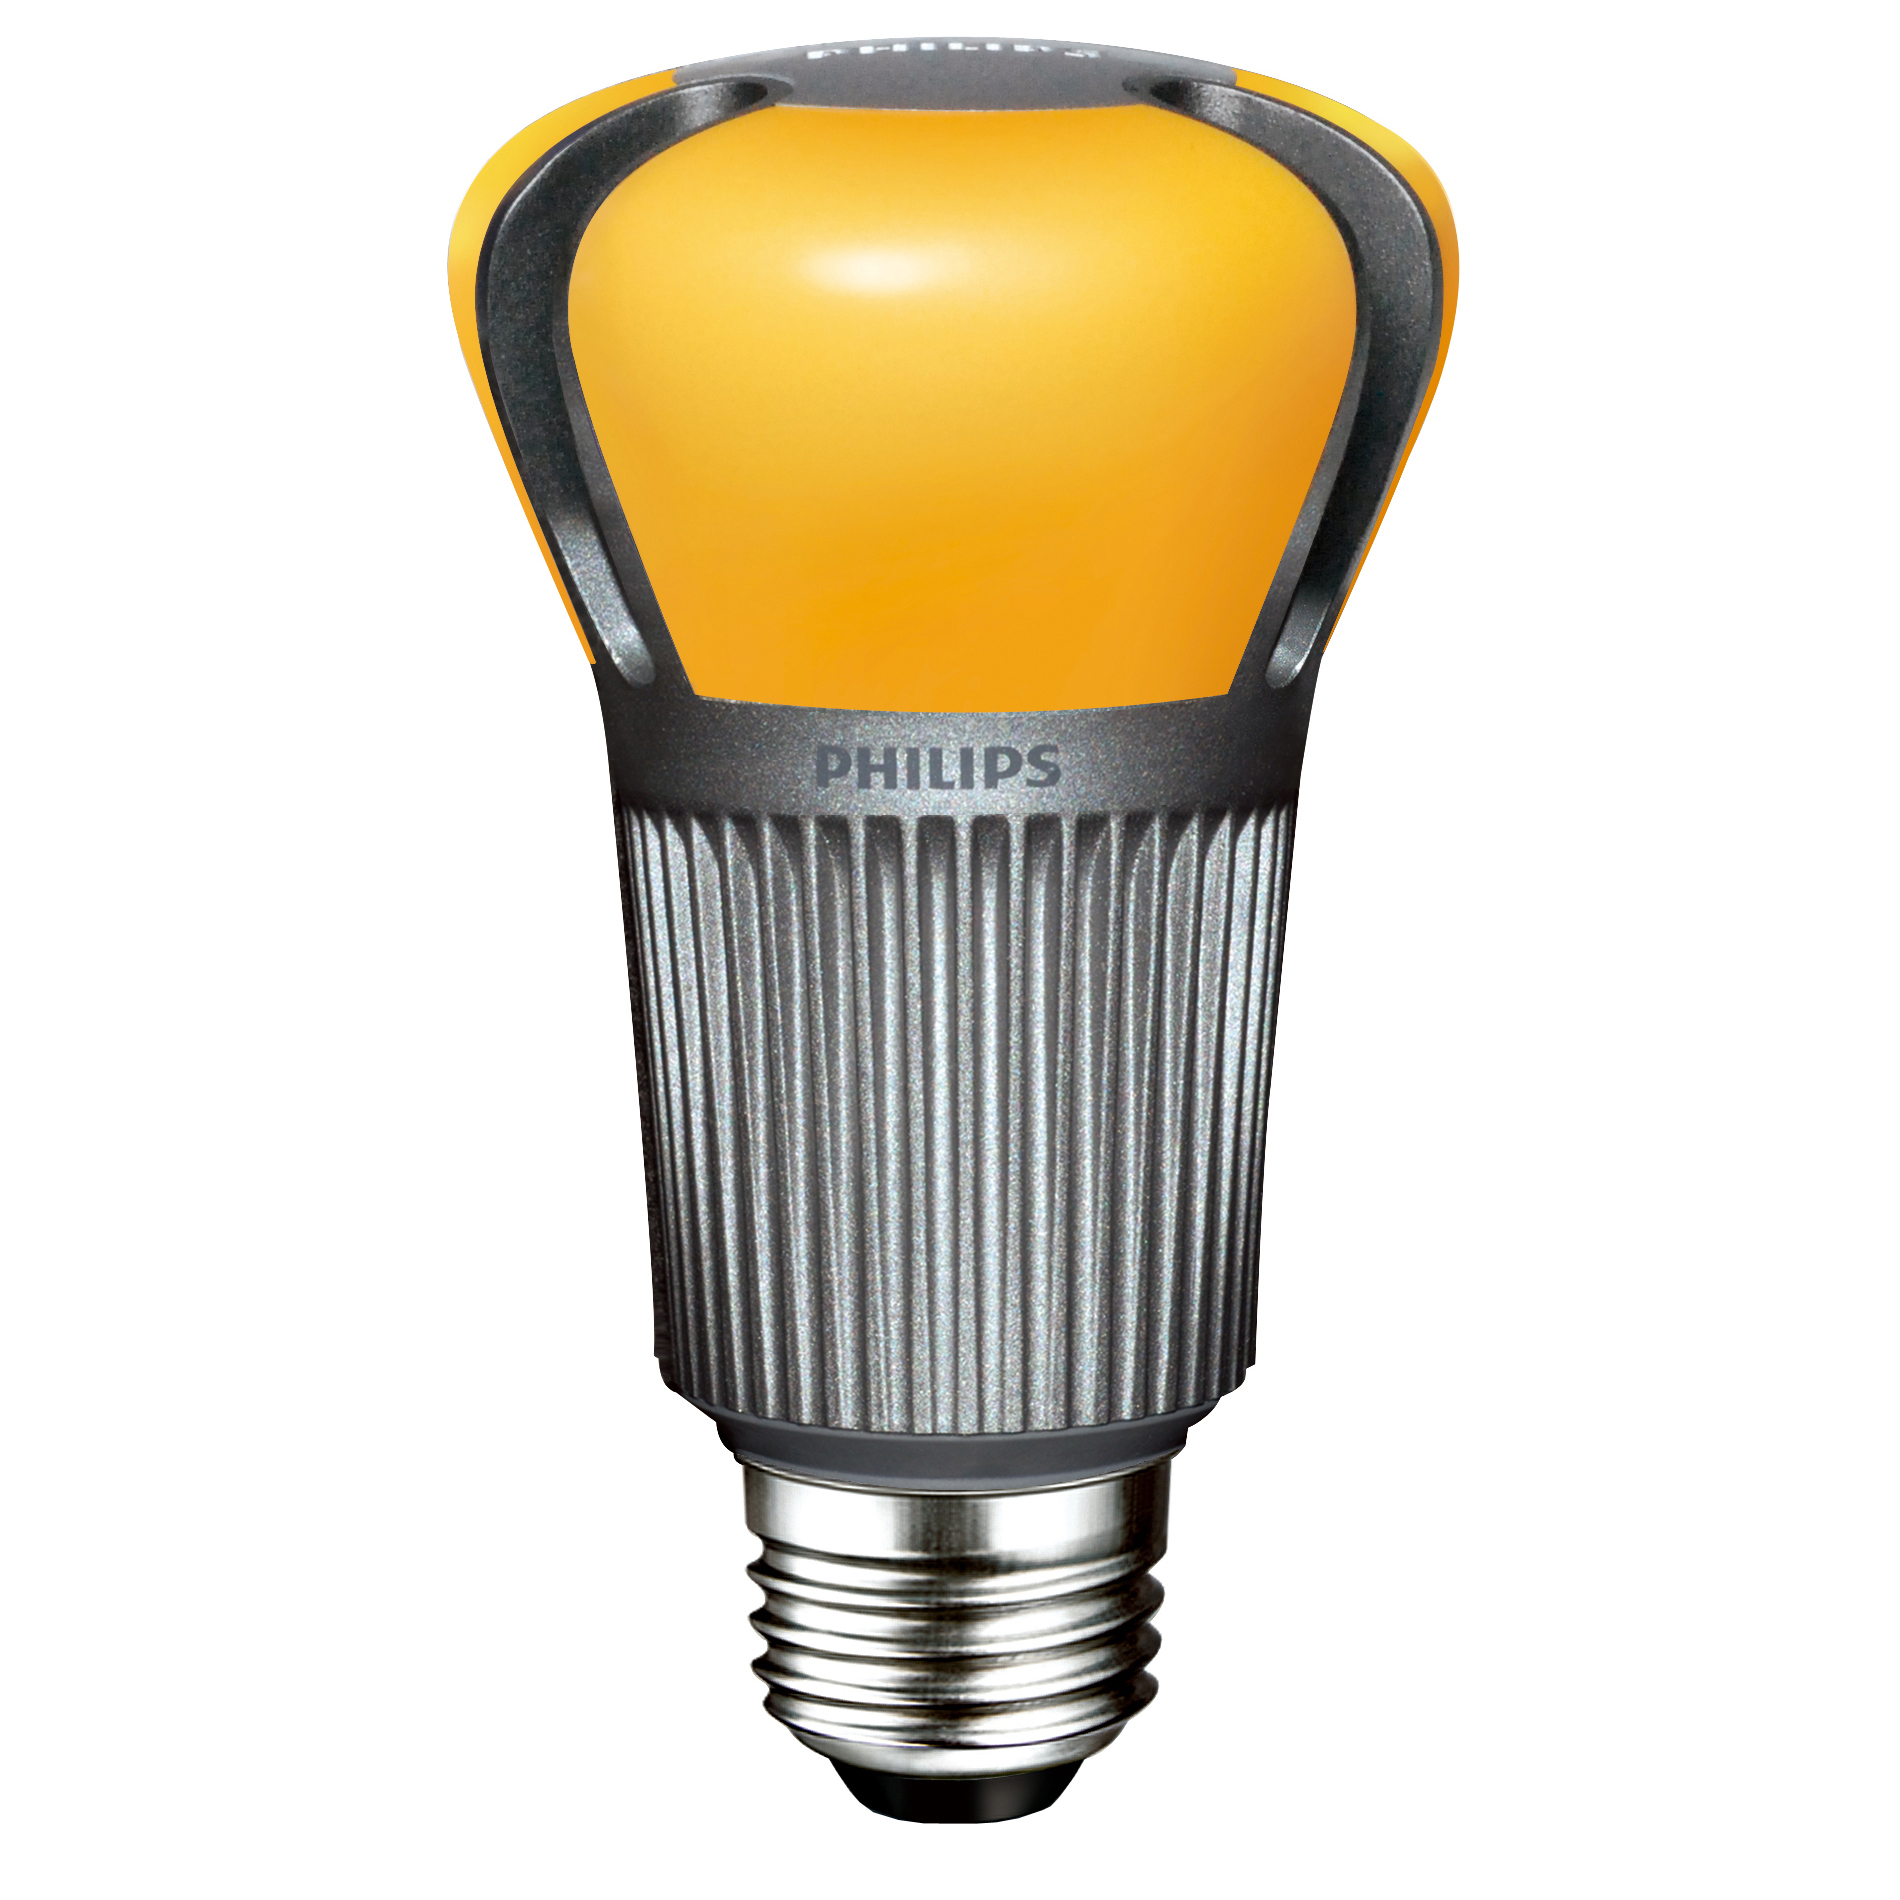
\includegraphics[width=4cm]{./0_intro/img/enduraled-12w.jpg}
\label{fig:l_prize}
\caption{900 lumens LED light bulb.}
\end{figure}

Two factors can be identified to make more favorable the adoption of the SSL as the preferred lighting solution by the consumers. In the one hand, reducing the end product price; and in the other hand, bringing more value to the traditional light sources. Actually LED light bulbs already bring more value compared to the old light bulbs being much more efficient, almost one order of magnitude lower in power consumption, and a longer lifetime, easily twenty times more operating hours. However these factors are not yet a valuable argument for the consumers. With the current trend of the \emph{internet-of-things} remote control, color tuning, light level dimming and integration to with future smart houses are probably some value propositions that people will need and SSL can easily provide. In a second level, I assume that the luminaries designs will change with a more favorable designs that take advantage of the low profiles of the LEDs.
 
 \begin{figure}[!h]
\centering
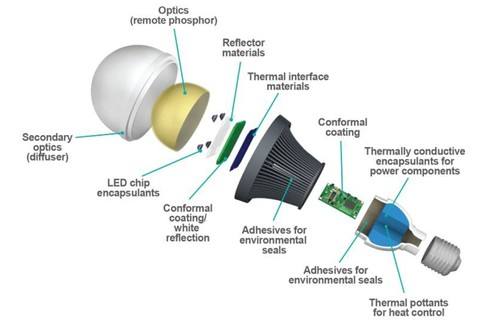
\includegraphics[width=4cm]{./0_intro/img/exploded_bulb_2.jpg}
\caption{900 lumens LED light bulb.}
\label{fig:exploded_bulb}
\end{figure}
 
It is essential to describe the different elements in a LED light bulb in order to understand the challenges in its development and  design. A LED light bulb is composed by the six main elements described below and shown in  the Fig. ~\ref{fig:exploded_bulb}. 

\begin{description}
  \item[LED] A two-lead semiconductor device that produced light when a current flows through it. The name comes from its acronym \emph{Light-Emitting Diode}. The light is produced by electroluminescence when an electron recombines with an electron-hole releasing energy in form of photons. The color of the light is determined by the energy band gap of the semiconductor.  
      
   LED cost is very cheap and there is a broad assortment in colors, power and applications. The selection of the LED will determine: light color, voltage and current of the load, efficiency and necessary optics. 
         
  \item[Optics] The optical device that helps to collimate, mix and distribute the light in the space in a desired way, normally uniformly for a determined projection area.  
     
  \item[Driver] Electronic circuit placed between the input source and the load, the LEDs, that transforms the input electrical power to the requirements of the load. Since almost all the power distribution systems and storage devices are voltage sources and LEDs are current supplied loads, an LED driver is considered as current-to-voltage (V-I) power supply. 
      
      The driver controls the current thought the load, hence the light output. Therefore it can be considered as the active part of the system where the control of the lamp relies. It is the most expensive and takes the largest volume of the lamp, and also one of the most or even the most important element in the entire system.
  
  \item[Heat sink] Mechanical element that acts as a passive heat exchanger and cools hot elements within the lamps system by dissipating the heat into the surrounding medium. The energy that is not converted to light becomes heat and must be extracted from the lamp, the main heat contributors elements are the LEDs and some components of the driver.
      
      The costs of the heat sink is also a relevant part in the total cost of the lamp.    
      
  \item[Body assembly] Mechanical element that hold all the different subsystems in one single device. In many cases the heat sink does this functionality. 
  
  \item[Connector] Mechanical element that provides connection with the energy source. The most popular one is the Edison connector present in all screw-in lamps. There are many other popular ones such as GU10, MR16, MR11 coming from the halogen multifaceted reflector bulbs or the 2-pin connector of the fluorescent tubes. 
      
      In many cases, the standardized connectors suppose a restriction for the mechanical design of the lamp. Their old-fashioned design is not optimal for the new lamps.
          
  
\end{description}

The chart shown in Fig.~\reg{fig:cost_breakdon} makes evident that the driver is the most expensive part of the system. As it was previously mentioned, the driver is the key component in the functionality of the LED lamp, since it controls the light output and at the same time determines the efficiency of the system. Therefore, the LED driver has become on of the hot topics of research within the power electronics field. Besides the necessity of fulfilling the operational requirements, such as high efficacy an proper power quality, two main issues have trigger research around the driver circuit: The costs and the volume. 

 


 \begin{figure}[!h]
\centering
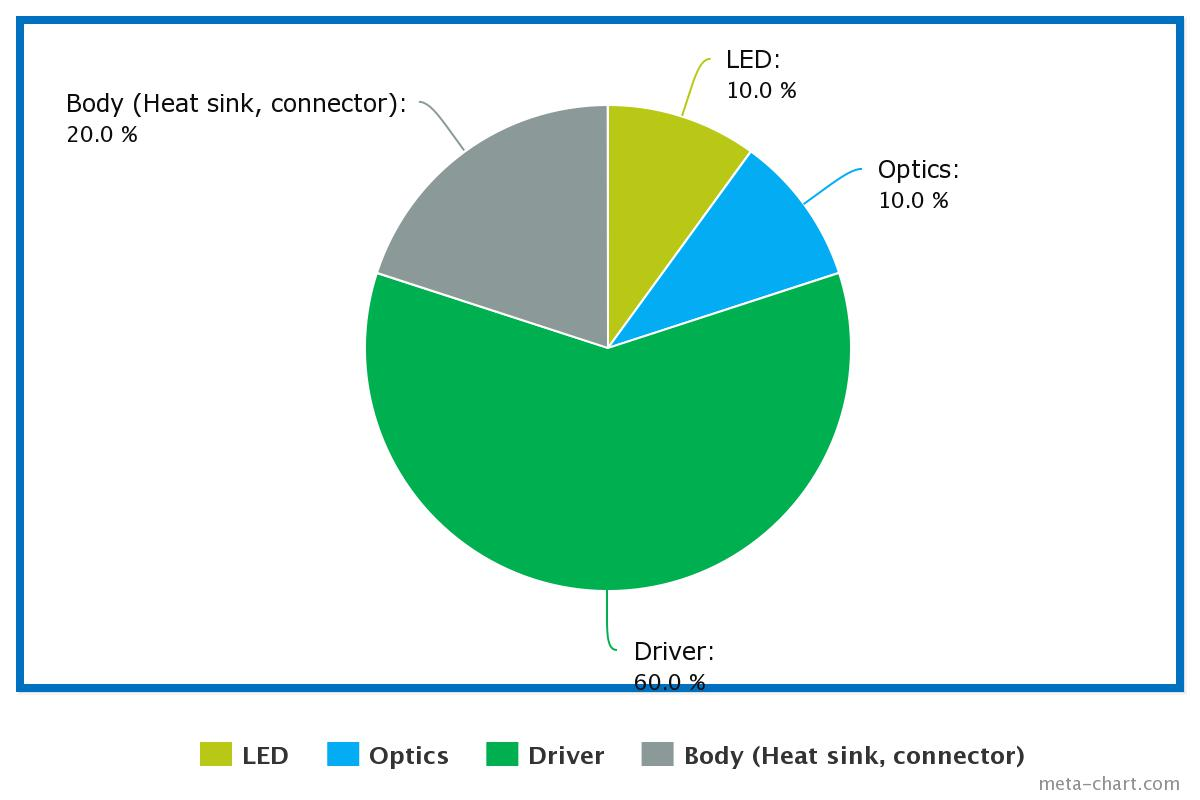
\includegraphics[width=4cm]{./0_intro/img/piechar_costs.jpeg}
\caption{LED lamp cost breakdown by subsystems.}
\label{fig:cost_breakdown}
\end{figure}


This section will make a little dissertation about what is the way to go:
\begin{enumerate}
  \item Cost driven driver production the cheapest the better
  \item Miniaturization + smart driver integration
\end{enumerate}

this section should gasp the current efforts done in order to introduce the LED light to the market. And say that the present way is retrofitting.

The section should close facing the dilemma that once the retrofitting is done where it will be the new market cases, and point that highly integrated drivers
can be one of the possible scenarios where integration and connectivity are part of a single solution.

%\chapter{An overview in LED driving}
%\section{DC-DC Drivers}
%\section{AC-DC Drivers}

\chapter{Introducing switched capacitors in LED drivers}
Presenting the concept of using a SCC with an inductor in order to enable integration and reduction in the size of the inductor.



